\documentclass[11pt, addpoints, answers]{exam}

\usepackage{amsmath, amssymb}
\usepackage{xcolor}
\usepackage{drawstack}

\newcommand{\red}[1]{\textcolor{red}{#1}}

% For inserting code snippets.
\usepackage{listings}
\lstset{
    columns = fixed,
    basewidth = {0.5em},
    breaklines = true,
    backgroundcolor = \color{white},
    keywordstyle = \color[RGB]{40, 40, 255},
    numberstyle = \footnotesize\color{darkgray},
    commentstyle = \ttfamily\color{violet},
    basicstyle = \ttfamily,
    stringstyle = \ttfamily\color[RGB]{128, 0, 0},
    showstringspaces = false,
    language = {[11]C++},
    escapechar = \@
}
\lstnewenvironment{cpp}[1][]{\lstset{language = {[11]C++}, #1}}{}

\usepackage{tikz}

% headers, footers, titles
\newcommand{\CourseName}{CS101 Algorithms and Data Structures}
\newcommand{\HomeworkNO}{Homework 5}
\newcommand{\DueDate}{Due date: November 12, 2023, at 23:59}

\pagestyle{headandfoot}
\runningheadrule
\runningheader{\CourseName}{\HomeworkNO}{\DueDate}
\runningfooter{}{\thepage}{}

\title{
	\CourseName\\
	Fall 2023\\
	\HomeworkNO
}
\author{}
\date{\DueDate}

% formats of questions, choices, points, etc.
\qformat{\textbf\thequestion. (\totalpoints\ points) \thequestiontitle\hfill}
\pointname{'}
\CorrectChoiceEmphasis{\color{red}}
\SolutionEmphasis{\color{red}}

% We frequently use this font.
\newcommand{\ttt}{\texttt}
\newcommand{\bluett}[1]{\textcolor{blue}{\ttt{#1}}}

\begin{document}

\maketitle

\begin{enumerate}
    \item Please write your solutions in English.
    \item Submit your solutions to gradescope.com.
    \item Set your FULL name to your Chinese name and your STUDENT ID correctly in Account Settings.
    \item If you want to submit a handwritten version, scan it clearly. \ttt{CamScanner} is recommended.
    \item When submitting, match your solutions to the problems correctly.
    \item No late submission will be accepted.
    \item Violations to any of the above may result in zero points.
\end{enumerate}

\begin{questions}

    \newpage

    \titledquestion{Multiple Choices}

Each question has \textbf{one or more} correct answer(s). Select all the correct answer(s). For each question, you will get 0 points if you select one or more wrong answers, but you will get 1 point if you select a non-empty subset of the correct answers.

Write your answers in the following table.

%%%%%%%%%%%%%%%%%%%%%%%%%%%%%%%%%%%%%%%%%%%%%%%%%%%%%%%%%%%%%%%%%%%%%%%%%%%
% Note: The `LaTeX' way to answer a multiple-choices question is to replace `\choice'
% with `\CorrectChoice', as what you did in the first question. However, there are still
% many students who would like to handwrite their homework. To make TA's work easier,
% you have to fill your selected choices in the table below, no matter whether you use 
% LaTeX or not.
%%%%%%%%%%%%%%%%%%%%%%%%%%%%%%%%%%%%%%%%%%%%%%%%%%%%%%%%%%%%%%%%%%%%%%%%%%%

\begin{table}[htbp]
    \centering
    \begin{tabular}{|p{2cm}|p{2cm}|p{2cm}|p{2cm}|}
        \hline
        (a) & (b) & (c) & (d) \\
        \hline
        %%%%%%%%%%%%%%%%%%%%%%%%%%%%%%%%%%%%%%%%%%%%%%%%%%%%%%%%%%
        % YOUR ANSWER HERE.
        AD  & BCD & AB  & D    \\
        %%%%%%%%%%%%%%%%%%%%%%%%%%%%%%%%%%%%%%%%%%%%%%%%%%%%%%%%%%
        \hline
    \end{tabular}
\end{table}

\begin{parts}
    \part[2] Which of the following operations on a \textbf{Linked List} take constant time?

    \begin{choices}
        \CorrectChoice Given a pointer $h$ which points  to the head node of a linked list, we want to erase the head node.
        \choice Given a pointer $h$ which points to the head node of a linked list, we want to gain access to the last element of the linked list.
        \choice Given a pointer $p$ which points to a node in a linked list, we want to gain access the previous node of $p$.
        \CorrectChoice Given a pointer $p$ which points to a node in a linked list, we want to insert an element after $p$.
    \end{choices}

    \part[2] Which of the following statements about arrays and linked-lists are true?

    \begin{choices}
        \choice Inserting an element into the middle of an array takes constant time.
        \CorrectChoice A doubly linked list consumes more memory than a (singly) linked list of the same length.
        \CorrectChoice Given a pointer to some node in a doubly linked list, we are able to gain access to every node of it.
        \CorrectChoice Given a pointer to any node in a linked list, we are able to gain access to the last node.
    \end{choices}

    \part[2] Please evaluate the following reverse-Polish expressions. Which of them are legal reverse-Polish expressions and gives a result greater than 0?

    \begin{choices}
        \CorrectChoice \ttt{2 3 2 * + 1 /}
        \CorrectChoice \ttt{1 2 4 - - 3 *}
        \choice \ttt{1 * 2 - 1 + 5}
        \choice \ttt{2 4 3 1 + * -}
    \end{choices}

    \part[2] Assume we implement a queue with a circular array indexed from $0$ to $n-1$. Now the \ttt{front} pointer is at index $a$, and the \ttt{back} pointer is at index $b$. Which of the following best describes the number of the elements in the queue?

    \begin{choices}
        \choice $b-a+1$
        \choice $|b-a+1|$
        \choice $b-a+1+n$
        \CorrectChoice $(b-a+1+n) \mod n$
    \end{choices}


\end{parts}

    \newpage

    %! Author = sutingchen
%! Date = 2023/10/18

\titledquestion{Generate a binary tree}

\begin{parts}
    \part[4] Given the in-order and pre-order traversal of a binary tree T are \textbf{ECFBDGA} and \textbf{ABCEFDG} respectively.\\
    Draw the tree T.\\
    \begin{solution} \\
        %\vspace{15em}
        \begin{center}
            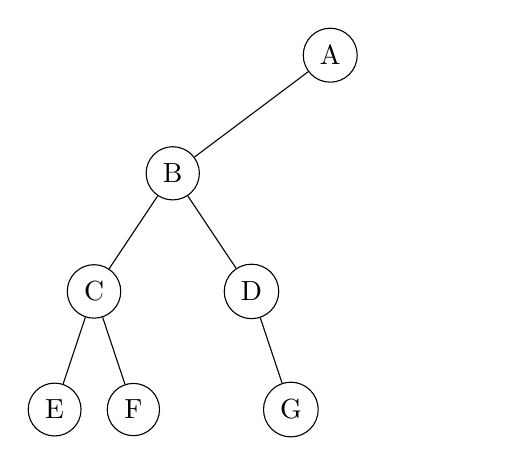
\begin{tikzpicture}[level distance=1.5cm,
                    level 1/.style={sibling distance=4cm},
                    level 2/.style={sibling distance=2cm},
                    level 3/.style={sibling distance=1cm},
                    every node/.style = {draw, circle}]
                \node {A}
                child { node {B}
                        child { node {C}
                                child { node {E} }
                                child { node {F} }
                            }
                        child { node {D}
                                child { edge from parent[draw=none] }
                                child { node {G} }
                            }
                    }
                child { edge from parent[draw=none] };
            \end{tikzpicture}
        \end{center}
    \end{solution}
    \vspace{2cm}
    \part[4] Given the in-order and post-order traversal of a binary tree T are \textbf{EBDAHCGF} and \textbf{EDBHFGCA} respectively.\\
    Draw the tree T.\\
    \begin{solution} \\
        %\vspace{15em}
        \begin{center}
            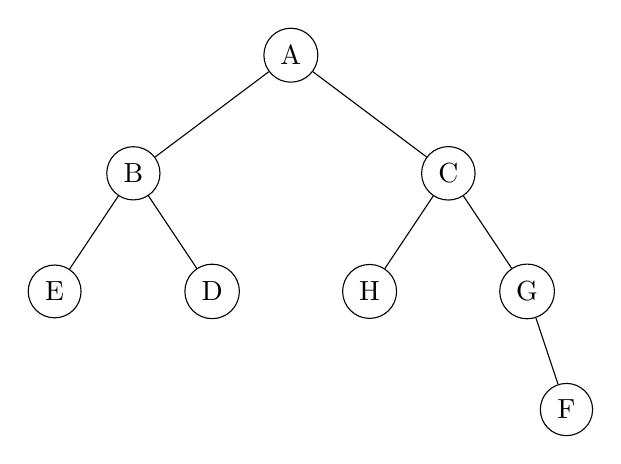
\begin{tikzpicture}[level distance=1.5cm,
                    level 1/.style={sibling distance=4cm},
                    level 2/.style={sibling distance=2cm},
                    level 3/.style={sibling distance=1cm},
                    every node/.style = {draw, circle}]
                \node {A}
                child { node {B}
                        child { node {E} }
                        child { node {D} }
                    }
                child { node {C}
                        child { node {H} }
                        child { node {G}
                                child { edge from parent[draw=none] }
                                child { node{F} }
                            }
                    };
            \end{tikzpicture}
        \end{center}
    \end{solution}
    % \vspace{2cm}
    \pagebreak
    \part[2] Given the pre-order and post-order traversal of a binary tree T, can you decide the tree T? If yes, please describe an algorithm to construct T; if no, please provide a counterexample.\\
    \begin{solution} \\
        %\vspace{20em}
        Knowing the pre-order and the post-order, we can construct the tree. \\
        \begin{enumerate}
            \item The first element in the pre-order and the last element in the post-order is the same,
                  which is the root. Remove it.
            \item The second element in the pre-order is the first children of the first element,
                  thus in the post-order elements in front of it form a subtree.
            \item Regard the subtree as a new tree and repeat the operations above.
            \item If facing with the elements shares the same position in pre-order and post-order,
                  this element is a leaf. For example, if ACB is the pre-order and ABC is the post-order,
                  A will be the leaf of the tree. Remove it.
        \end{enumerate}

    \end{solution}
\end{parts}

    \newpage

    \titledquestion{Tree Structure and Traversal}

\newcommand{\stack}[5]{
    \begin{minipage}{.13\linewidth}
        \begin{tikzpicture}[scale=0.5]
            \cell{#1}
            \cell{#2}
            \cell{#3}
            \cell{#4}
            \cell{#5}
        \end{tikzpicture}
    \end{minipage}
}

You should solve the below questions following these steps:
\begin{enumerate}
    \item Decide on an appropriate \textbf{data structure} to implement the traversal.
    \item When doing \textbf{Breadth First Traversal}, push children of a node into the data structure in alphabetical order.
    \item Consider \textbf{poping an entry} and \textbf{pushing all its children} as one step.
\end{enumerate}

\textbf{Example: }
Given a tree with root \textbf{A}: \\
\begin{figure}[h]
    \centering
    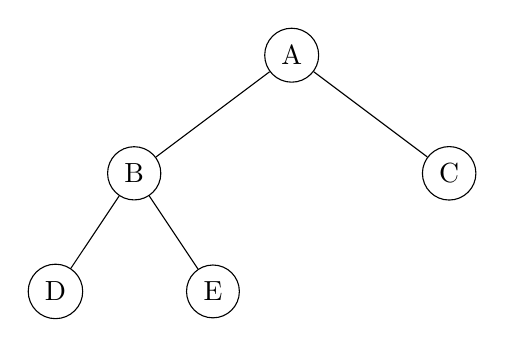
\begin{tikzpicture}[level distance=1.5cm,
            level 1/.style={sibling distance=4cm},
            level 2/.style={sibling distance=2cm},
            every node/.style = {draw, circle}]
        \node {A}
        child { node {B}
                child { node {D} }
                child { node {E} }
            }
        child { node {C} };
    \end{tikzpicture}
    \label{fig:example_pic}
\end{figure}

The process of doing \textbf{Breadth First Traversal} is: \\

\begin{figure}[h]
    \centering
    \stack{}{}{}{}{A} $\to$
    \stack{}{}{}{C}{B} $\to$
    \stack{}{}{E}{D}{C} $\to$
    \stack{}{}{}{E}{D} $\to$
    \stack{}{}{}{}{E} $\to$
    \stack{}{}{}{}{}
    \label{fig:example_sol}
\end{figure}

\pagebreak
\begin{parts}

    \part[5] Run \textbf{Breadth First Traversal} on the tree with root \textbf{A} and draw the whole process in the space below.

    \begin{figure}[h]
        \centering
        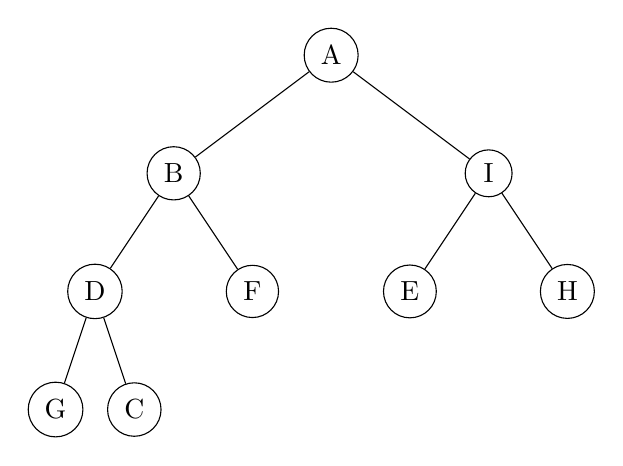
\begin{tikzpicture}[level distance=1.5cm,
                level 1/.style={sibling distance=4cm},
                level 2/.style={sibling distance=2cm},
                level 3/.style={sibling distance=1cm},
                every node/.style = {draw, circle}]
            \node {A}
            child { node {B}
                    child { node {D}
                            child { node {G} }
                            child { node {C} }
                        }
                    child { node {F} }
                }
            child { node {I}
                    child { node {E} }
                    child { node {H} }
                };
        \end{tikzpicture}
        \label{fig:traversal_question_1}
    \end{figure}

    \begin{solution} \\
        %\vspace{30em}
        Breadth First Traversal can be implemented by queue.
        The process of doing \textbf{Breadth First Traversal} is: \\
        \begin{center}
            \stack{}{}{}{}{A} $\to$
            \stack{}{}{}{I}{B} $\to$
            \stack{}{}{F}{D}{I} $\to$
            \stack{}{H}{E}{F}{D} $\to$
            \stack{G}{C}{H}{E}{F} $\to$
            \stack{}{G}{C}{H}{E} $\to$
            \stack{}{}{G}{C}{H} $\to$
            \stack{}{}{}{G}{C} $\to$
            \stack{}{}{}{}{G} $\to$
            \stack{}{}{}{}{}
        \end{center}
    \end{solution}

    \pagebreak
    \part[5] Run \textbf{Pre-order Depth First Traversal} on the tree with root \textbf{A} and draw the whole process in the space below.

    \begin{figure}[h]
        \centering
        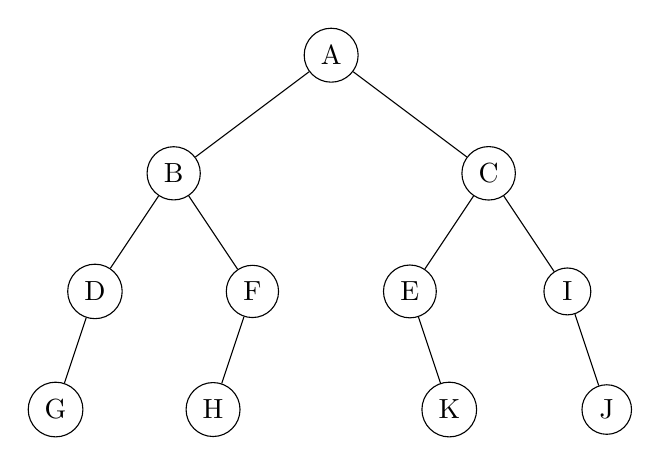
\begin{tikzpicture}[level distance=1.5cm,
                level 1/.style={sibling distance=4cm},
                level 2/.style={sibling distance=2cm},
                level 3/.style={sibling distance=1cm},
                every node/.style = {draw, circle}]
            \node {A}
            child { node {B}
                    child { node {D}
                            child { node {G} }
                            child { edge from parent[draw=none] }
                        }
                    child { node {F}
                            child { node {H} }
                            child { edge from parent[draw=none] }
                        }
                }
            child { node {C}
                    child { node {E}
                            child { edge from parent[draw=none] }
                            child { node {K} }
                        }
                    child { node {I}
                            child { edge from parent[draw=none] }
                            child { node {J} }
                        }
                };
        \end{tikzpicture}
        \label{fig:traversal_question_2}
    \end{figure}

    \begin{solution}
        %\vspace{30em}
        It can be implemented by stack.
        The process of doing \textbf{Pre-order Depth First Traversal} is: \\
        \begin{center}
            \stack{}{}{}{}{A} $\to$
            \stack{}{}{}{B}{C} $\to$
            \stack{}{}{D}{F}{C} $\to$
            \stack{}{}{G}{F}{C} $\to$
            \stack{}{}{}{F}{C} $\to$
            \stack{}{}{}{H}{C} $\to$
            \stack{}{}{}{}{C} $\to$
            \stack{}{}{}{E}{I} $\to$
            \stack{}{}{}{K}{I} $\to$
            \stack{}{}{}{}{I} $\to$
            \stack{}{}{}{}{J} $\to$
            \stack{}{}{}{}{}
        \end{center}
    \end{solution}

    \pagebreak
\end{parts}

    \newpage

    %! Author = sutingchen
%! Date = 2023/10/20

\titledquestion{Left Child Right Sibling}

\begin{parts}
    \part[1] For every ordered tree, there is a unique representation of Left-child right-sibling format.

    \begin{oneparcheckboxes}
        \CorrectChoice True
        \choice False
    \end{oneparcheckboxes}

    \part[1] Pre-order traversal of the original tree is identical to the pre-order traversal of the Knuth transform.

    \begin{oneparcheckboxes}
        \CorrectChoice True
        \choice False
    \end{oneparcheckboxes}

    \part[1] Post-order traversal of the original tree is identical to the post-order traversal of the Knuth transform.

    \begin{oneparcheckboxes}
        \choice True
        \CorrectChoice False
    \end{oneparcheckboxes}


    \part[7] Transform the tree below with root \textbf{1} (in LCRS format) to N-ary format.

    \begin{figure}[h]
        \centering
        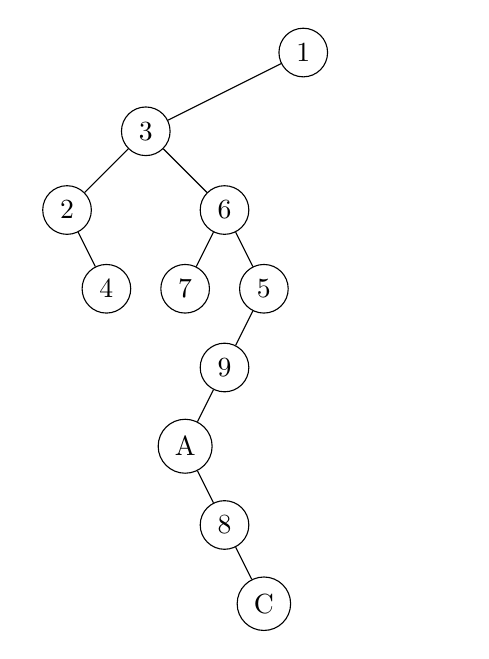
\begin{tikzpicture}[level distance=1cm,
                level 1/.style={sibling distance=4cm},
                level 2/.style={sibling distance=2cm},
                level 3/.style={sibling distance=1cm},
                every node/.style = {draw, circle}]
            \node {1}
            child { node {3}
                    child { node {2}
                            child { edge from parent[draw=none] }
                            child { node {4} }
                        }
                    child { node {6}
                            child { node {7} }
                            child { node {5}
                                    child { node {9}
                                            child { node {A}
                                                    child { edge from parent[draw=none] }
                                                    child { node {8}
                                                            child { edge from parent[draw=none] }
                                                            child { node {C} }
                                                        }
                                                }
                                            child { edge from parent[draw=none] }
                                        }
                                    child { edge from parent[draw=none] }
                                }
                        }
                }
            child { edge from parent[draw=none] };
        \end{tikzpicture}

        \label{fig:LCRS_question}
    \end{figure}

    \begin{solution}
        %\vspace{10em}
        \begin{center}
            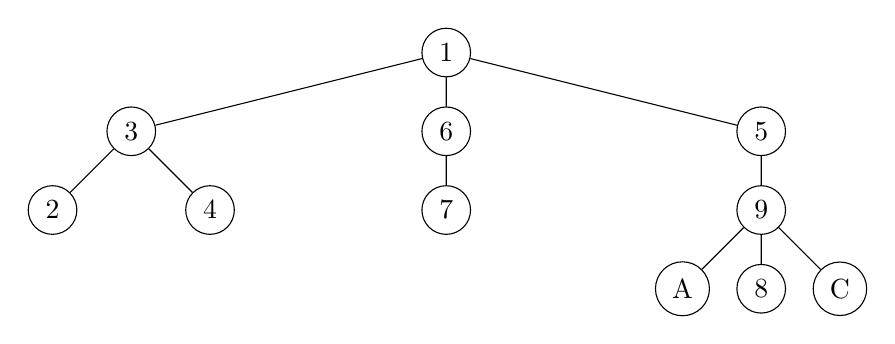
\begin{tikzpicture}[level distance=1cm,
                    level 1/.style={sibling distance=4cm},
                    level 2/.style={sibling distance=2cm},
                    level 3/.style={sibling distance=1cm},
                    every node/.style = {draw, circle}]
                \node {1}
                child { node {3}
                        child { node {2} }
                        child { node {4} }
                    }
                child { node {6}
                        child { node {7} }
                    }
                child { node {5}
                        child { node {9}
                                child { node {A} }
                                child { node {8} }
                                child { node {C} }
                            }
                    };
            \end{tikzpicture}
        \end{center}
    \end{solution}

\end{parts}


\end{questions}

\end{document}